\documentclass[a4paper,11pt]{article}
\usepackage[utf8]{inputenc}
\usepackage[T1]{fontenc}
\usepackage{helvet}\renewcommand{\familydefault}{\sfdefault}
\usepackage[a4paper,top=2.2cm,bottom=2.2cm,left=2.3cm,right=2.3cm]{geometry}
\usepackage{graphicx}
\usepackage{xcolor}
\usepackage{array}
\usepackage{longtable}
\usepackage{enumitem}
\usepackage{titlesec}
\usepackage{fancyhdr}
\usepackage[hidelinks]{hyperref}
\usepackage{tcolorbox}

\definecolor{azul}{HTML}{1F4E79}
\definecolor{cinza}{HTML}{5A5A5A}
\definecolor{fundo}{HTML}{EEF3F8}
\renewcommand{\figurename}{Figura}
\renewcommand{\tablename}{Tabela}
\renewcommand{\contentsname}{Sumário}
\setlength{\parindent}{0pt}
\setlength{\parskip}{5pt}
\setlist{itemsep=2pt,topsep=3pt}
\titleformat{\section}{\Large\bfseries\color{azul}}{\thesection.}{0.6em}{}
\titleformat{\subsection}{\large\bfseries\color{azul}}{\thesubsection.}{0.5em}{}
\pagestyle{fancy}\fancyhf{}
\lhead{\small\color{cinza}Projeto de Banco de Dados -- Oficina Mecânica}
\rhead{\small\color{cinza}Resumo e roteiro da apresentação}
\cfoot{\small\thepage}
\renewcommand{\headrulewidth}{0.3pt}
\newcommand{\cod}[1]{\texttt{\small #1}}
\newtcolorbox{caixa}[1][]{colback=fundo,colframe=azul,boxrule=0.6pt,arc=2pt,left=6pt,right=6pt,top=4pt,bottom=4pt,#1}

\begin{document}

\begin{center}
{\color{azul}\Huge\bfseries Oficina Mecânica}\\[4pt]
{\Large Projeto de Banco de Dados -- Unidade II -- Tema 07}\\[10pt]
{\large Resumo do que foi feito e roteiro da apresentação}\\[10pt]
\textbf{Equipe:} Jarlisson Brito Santos, Brunno Passos, Caio Vinicius\\[2pt]
\textbf{Apresentação:} 30/11/2026 -- 10 minutos por grupo (15h10 às 18h30)\\[2pt]
\textbf{Repositório:} \url{https://github.com/Jarlisson-cpu/oficina-mecanica--bd}
\end{center}

\vspace{4pt}
\tableofcontents
\vspace{6pt}

\begin{caixa}
\textbf{Resumo em uma frase.} Montamos um banco de dados em PostgreSQL que
impede os erros mais comuns de uma oficina mecânica (placa duplicada, peça
usada sem baixa no estoque, OS sem responsável, hodômetro voltando e OS fechada
sendo alterada) e provamos cada regra com teste: \textbf{34 de 34 testes
passaram} e os índices deixaram a busca por placa \textbf{cerca de 120 vezes mais
rápida} (30,60~ms $\rightarrow$ 0,25~ms).
\end{caixa}

\newpage
% =====================================================================
\section*{Parte 1 -- O que foi feito}
\addcontentsline{toc}{section}{Parte 1 -- O que foi feito}

\section{O problema}
Na oficina, o controle em papel ou planilha gera falhas recorrentes. Cada
uma virou uma regra no banco e um teste:

\begin{longtable}{p{4.6cm}p{6.2cm}p{4.2cm}}
\hline
\textbf{Problema} & \textbf{Como o banco resolve} & \textbf{Teste que prova} \\ \hline
Placa ou CPF cadastrado duas vezes & \cod{UNIQUE} + domínios de formato & R02, R03, T02, T10 \\
Peça usada sem baixa no estoque & trigger de baixa/estorno + \cod{CHECK (qtd\_estoque >= 0)} & G01, G02, G08 \\
OS sem mecânico responsável & \cod{NOT NULL} + chave estrangeira + trigger ``mecânico ativo'' & G05 \\
Hodômetro ``voltando'' & trigger compara com o km já registrado & G06 \\
OS fechada sendo alterada & \cod{CHECK}s de data/status + trigger de ciclo de vida & R07--R09, G04, G07 \\
Histórico por placa demorado & índice \cod{(id\_veiculo, data\_abertura DESC)} & B1: 30,60 $\rightarrow$ 0,25 ms \\ \hline
\end{longtable}

\section{A solução (arquitetura e modelo)}
\begin{itemize}
  \item \textbf{SGBD:} PostgreSQL 16, schema \cod{oficina}.
  \item \textbf{6 tabelas:} \cod{cliente}, \cod{veiculo}, \cod{mecanico},
  \cod{ordem\_servico}, \cod{peca} e \cod{os\_peca} (associativa N:N entre OS e peça,
  com chave primária composta).
  \item \textbf{Domínios} (regra de formato escrita uma vez só): placa antiga e
  Mercosul, CPF/CNPJ só com dígitos, telefone, dinheiro e status como \cod{ENUM}.
  \item \textbf{5 regras de negócio em triggers:} copiar o preço da peça; bloquear
  alteração de OS fechada; baixa/estorno de estoque; mecânico ativo e hodômetro;
  ciclo de vida da OS e cálculo da mão de obra (horas $\times$ valor-hora).
  \item \textbf{View} \cod{vw\_os\_total}: valor de cada OS (peças + mão de obra $-$ desconto).
  \item \textbf{8 índices}, cada um ligado a uma consulta real da oficina.
  \item \textbf{Dados de teste:} 20 mil clientes, 30 mil veículos, 300 mil OS e
  450 mil itens de peça (fictícios, gerados por script).
\end{itemize}

\begin{figure}[h]
\centering
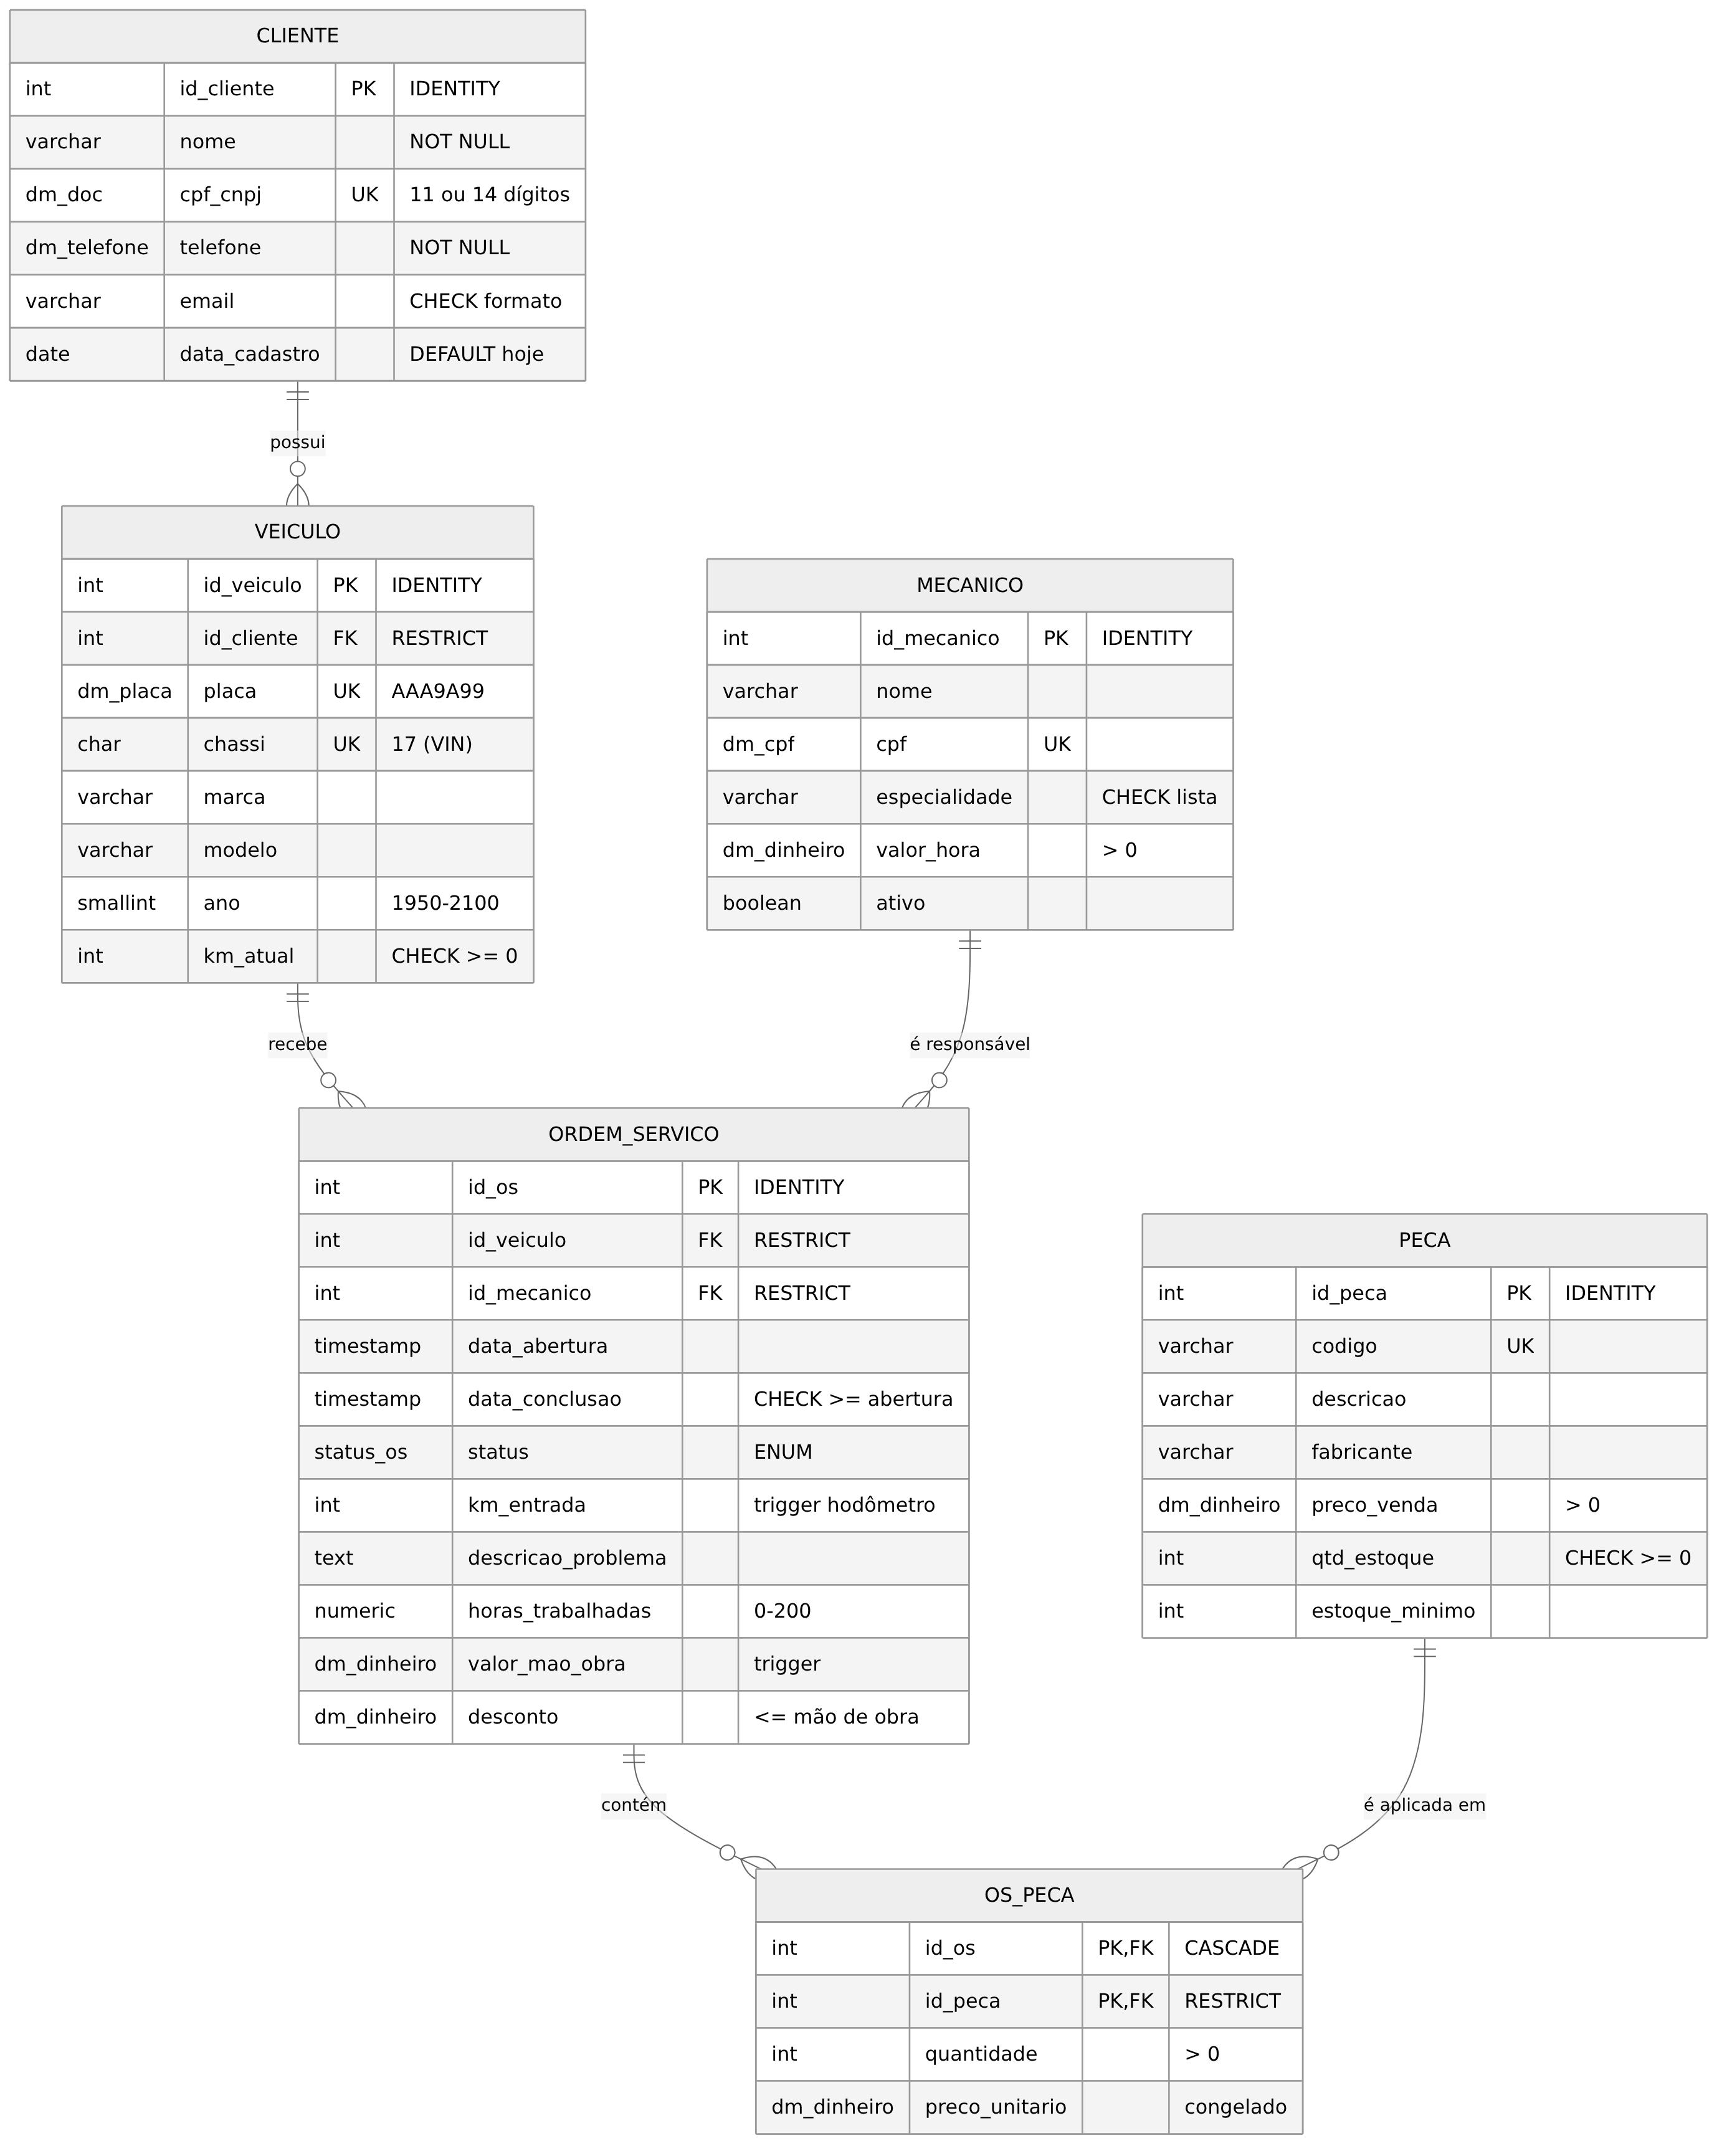
\includegraphics[width=.47\linewidth]{../diagramas/der.png}\hfill
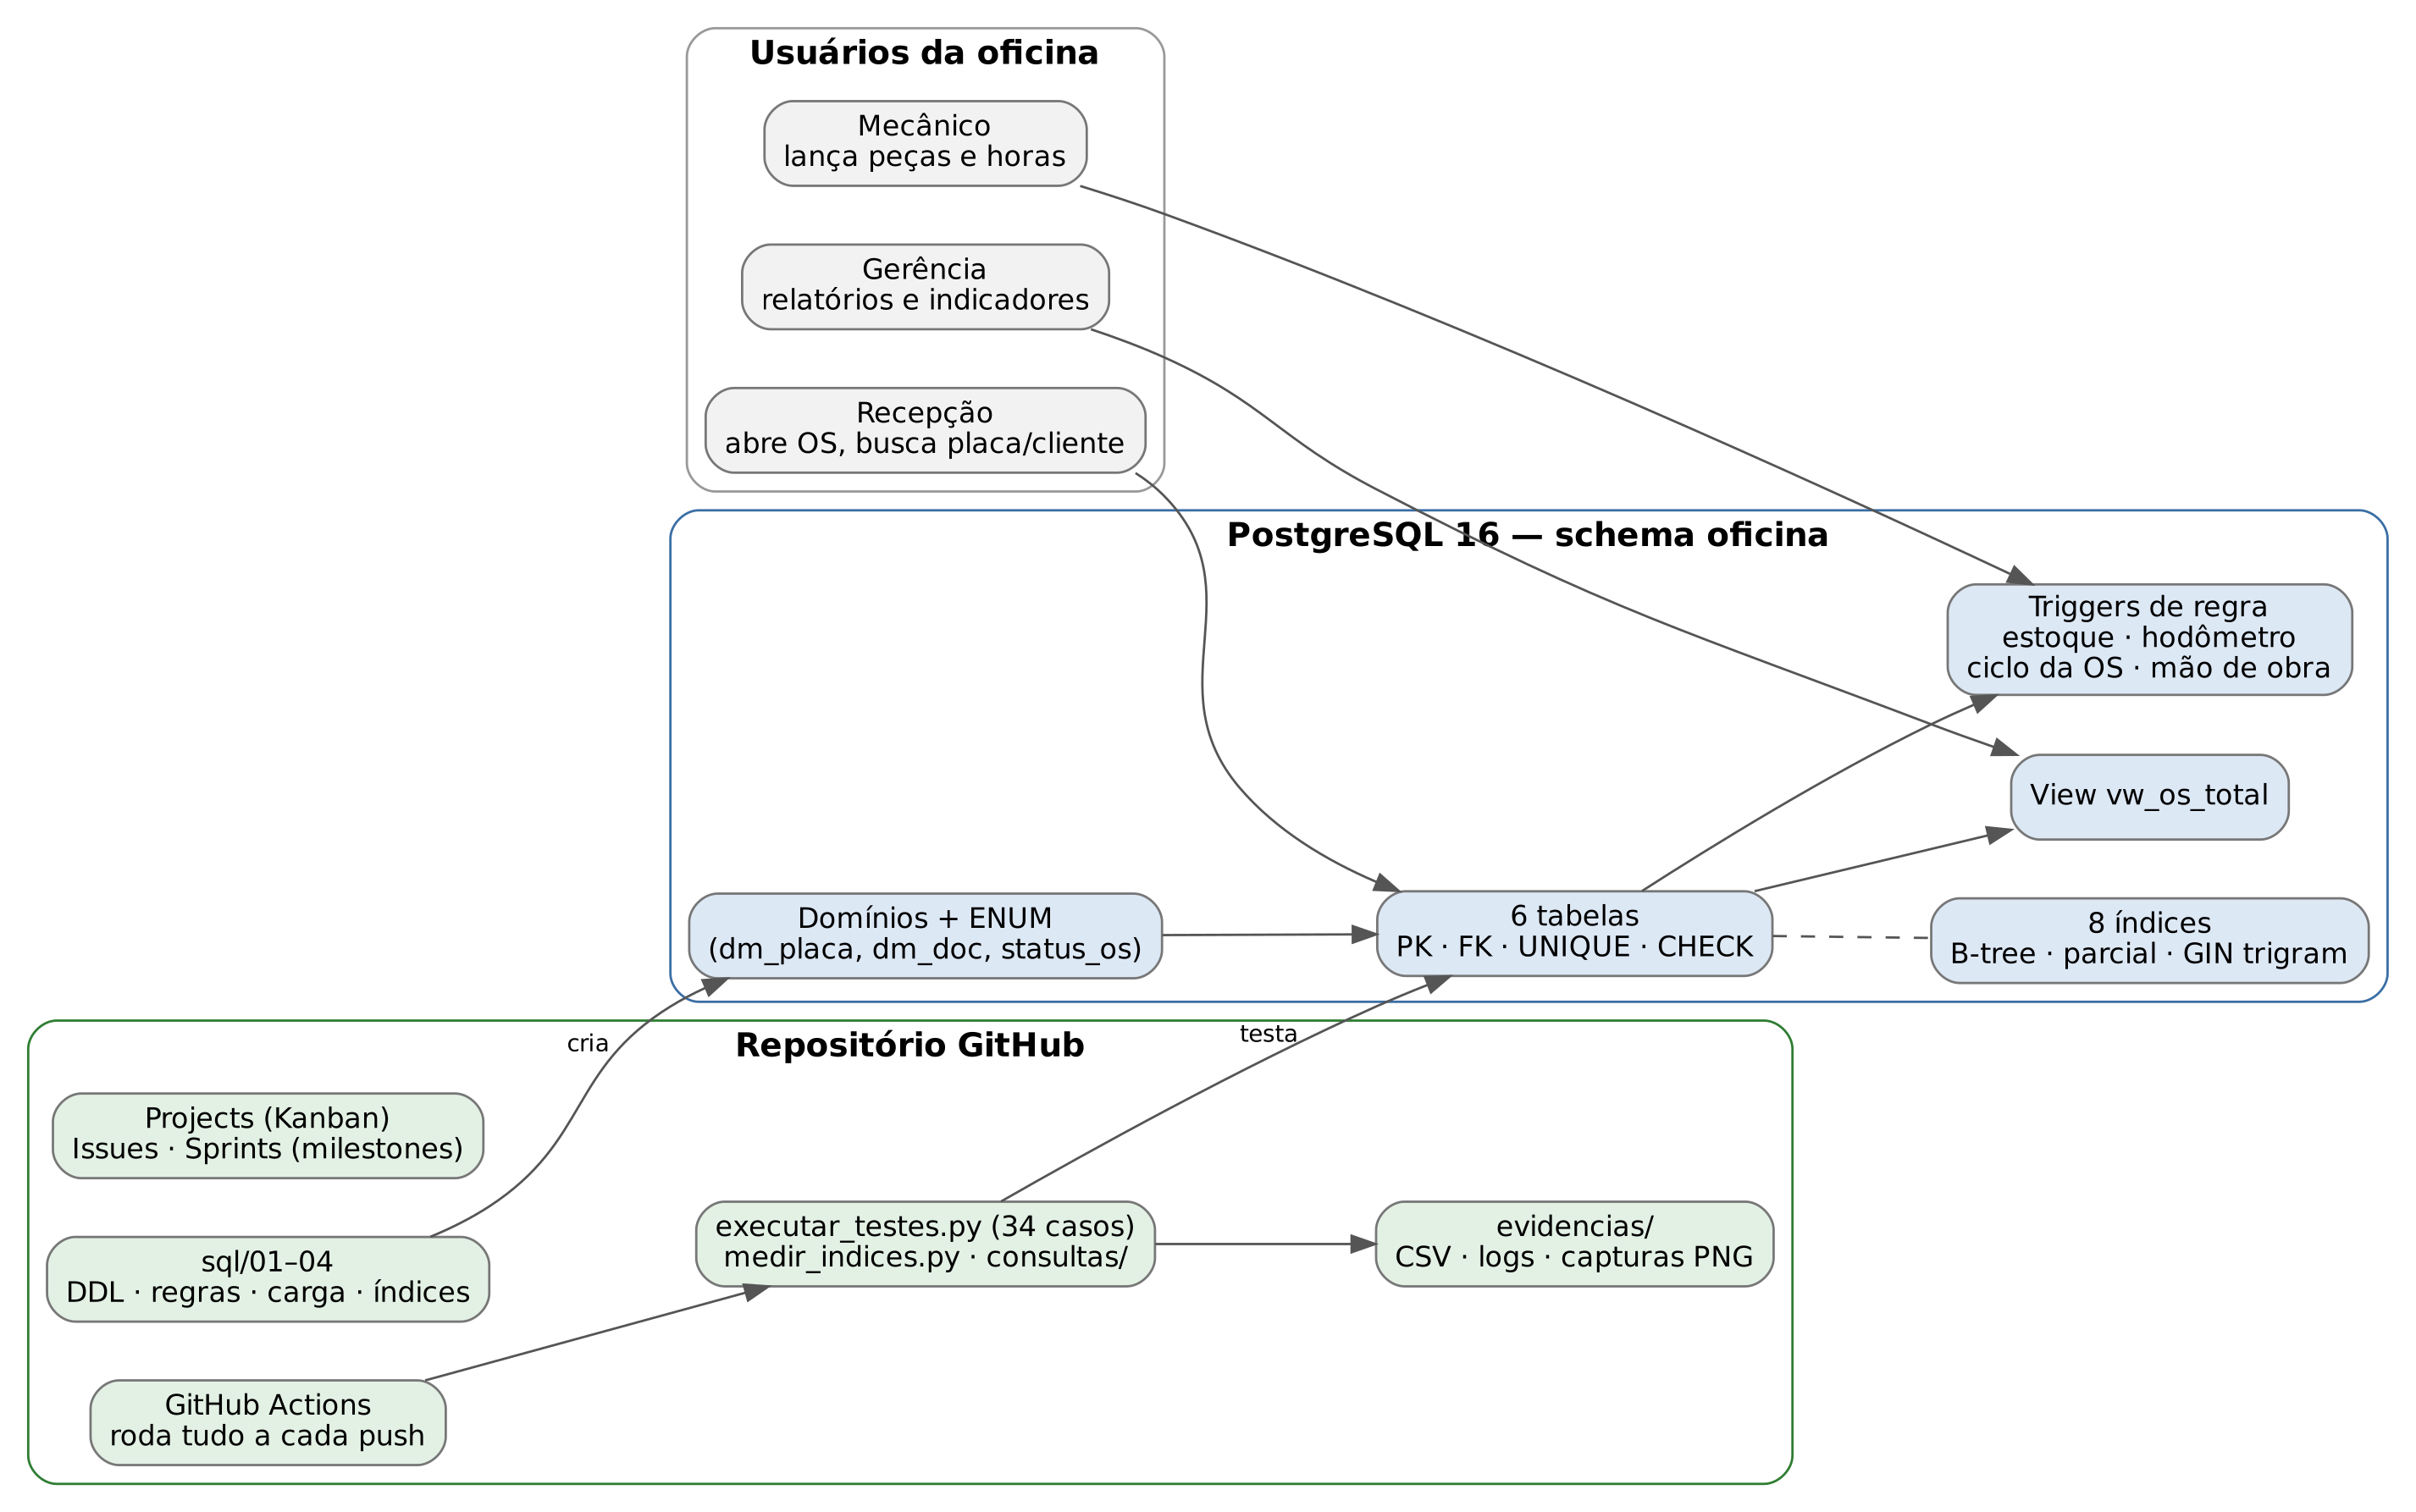
\includegraphics[width=.5\linewidth]{../diagramas/arquitetura.png}
\caption{Diagrama ER (esquerda) e arquitetura da solução (direita).}
\end{figure}

\section{Testes de tipos, restrições e regras}
\begin{itemize}
  \item \textbf{34 testes automatizados}: 11 de tipos (T), 13 de restrições (R) e
  10 de regras/triggers (G). \textbf{Todos passaram.}
  \item Nos 26 testes em que o banco deveria recusar o comando, ele devolveu
  \textbf{exatamente o código de erro esperado} (ex.: 23505 = valor duplicado,
  23503 = chave estrangeira, 23514 = CHECK).
  \item Cada teste roda dentro de \cod{BEGIN \dots{} ROLLBACK} (não suja o banco)
  e gera um log \cod{.txt} e uma captura de tela \cod{.png}.
  \item Destaques para mostrar: \textbf{T07} (\cod{FLOAT} erra $0{,}1+0{,}2$ e
  \cod{NUMERIC} não), \textbf{G02} (estoque insuficiente barrado) e \textbf{G10}
  (fluxo completo: abrir, lançar peças, concluir e faturar R\$~348,40).
\end{itemize}

\section{Índices: antes e depois}
Medido com \cod{EXPLAIN ANALYZE}, mediana de 7 execuções:

\begin{longtable}{p{5.4cm}rrp{4.1cm}}
\hline
\textbf{Consulta} & \textbf{Antes} & \textbf{Depois} & \textbf{Páginas lidas} \\ \hline
B1 Histórico por placa & 30,60 ms & 0,25 ms & 8.323 $\rightarrow$ 31 \\
B2 Painel de OS pendentes (índice parcial) & 24,80 ms & 0,35 ms & 8.276 $\rightarrow$ 52 \\
B3 Produção do mecânico no mês & 24,32 ms & 0,84 ms & 8.204 $\rightarrow$ 200 \\
B4 Faturamento do mês & 23,52 ms & 6,28 ms & 8.204 $\rightarrow$ 2.590 \\
B5 Consumo de uma peça & 29,25 ms & 2,56 ms & 2.870 $\rightarrow$ 611 \\
B6 Veículos de um cliente & 2,00 ms & 0,14 ms & 613 $\rightarrow$ 4 \\
B7 Cliente por parte do nome (GIN) & 12,04 ms & 0,97 ms & 266 $\rightarrow$ 174 \\
B8 OS concluídas (95\% da tabela) & 46,32 ms & 49,09 ms & \textbf{índice ignorado} \\
B9 OS abertas (0,2\% da tabela) & 25,46 ms & 1,59 ms & 8.204 $\rightarrow$ 532 \\
W1 Inserir 20 mil OS (custo de escrita) & 1.250 ms & 1.578 ms & +26\% mais lento \\ \hline
\end{longtable}

\textbf{O que aprendemos (resultados ``contra a intuição''):}
\begin{itemize}
  \item Índice em coluna com poucos valores diferentes (\cod{status}) é
  \textbf{ignorado} quando o filtro pega quase a tabela toda (B8), mas é usado quando pega pouco (B9).
  \item Índice tem custo: inserir ficou \textbf{26\% mais lento} e os índices ocupam cerca de 40 MB.
  \item A view com \cod{LATERAL} ficou \textbf{633$\times$ mais rápida} para uma placa,
  mas \textbf{2$\times$ mais lenta} no relatório geral; por isso o relatório geral soma direto nas tabelas.
  \item Os testes acharam um \textbf{erro numa consulta de estoque} (C04 somava todos os
  períodos); ele foi corrigido.
\end{itemize}

\section{Consultas de negócio (C01--C08)}
C01 histórico por placa; C02 faturamento mensal (tíquete médio entre R\$~748 e R\$~770);
C03 ranking de mecânicos (\cod{RANK()}); C04 peças para repor; C05 OS atrasadas;
C06 top 10 clientes; C07 taxa de retrabalho por mecânico (\cod{LAG()}, maior taxa 1,85\%);
C08 conferência: total da view = total das tabelas (R\$~216.799.627,25 nos dois).

\section{GitHub e metodologia ágil}
\begin{itemize}
  \item \textbf{Repositório público:} \url{https://github.com/Jarlisson-cpu/oficina-mecanica--bd}
  \item \textbf{Scrum simplificado} com 5 sprints semanais (\emph{Milestones}), até 30/11.
  \item \textbf{18 tarefas} (\emph{Issues}) com rótulos: 13 concluídas e 5 abertas.
  \item \textbf{GitHub Actions:} a cada envio o GitHub recria o banco e roda os 34 testes
  sozinho (selo verde no README).
  \item \textbf{Definição de pronto:} SQL no repositório + teste automatizado + evidência gerada.
\end{itemize}

\section{O que foi entregue e onde está}
Pasta \cod{Documentos\textbackslash Projeto BD - Oficina Mecanica}:
\begin{longtable}{p{5.2cm}p{9.8cm}}
\hline
\textbf{Pasta} & \textbf{Conteúdo} \\ \hline
00 - Enunciado e Modelos & enunciado do professor e modelos SBC \\
01 - Artigo & artigo em PDF, Word (.docx) e LaTeX (.tex) + figuras \\
02 - Banco de Dados & scripts SQL 01 a 04 e as consultas C01--C08 \\
03 - Testes e Evidencias & resumo dos testes, tabelas CSV, capturas, logs e planos de execução \\
04 - Diagramas & diagrama ER e arquitetura \\
05 - Repositorio GitHub & cópia compactada do repositório \\
06 - Resumo e Roteiro dos Slides & este documento \\ \hline
\end{longtable}

\section{O que ainda falta}
\begin{itemize}
  \item Preencher no artigo: \textbf{[Nome do(a) Professor(a)]} e \textbf{[Curso]}.
  \item Criar o \textbf{quadro Kanban} no GitHub (aba Projects) e adicionar
  \cod{caiosouza0121} e \cod{devebruzzz} como colaboradores (Settings $\rightarrow$ Collaborators).
  \item Montar os \textbf{slides} (roteiro na Parte 2) e \textbf{ensaiar} com cronômetro.
\end{itemize}

% =====================================================================
\newpage
\section*{Parte 2 -- O que vai ser apresentado nos slides}
\addcontentsline{toc}{section}{Parte 2 -- O que vai ser apresentado nos slides}

Tempo total: \textbf{10 minutos}, com 10 slides. A divisão por pessoa é uma sugestão;
ajustem como preferirem. Regra de ouro do professor: \emph{toda afirmação vem com um teste},
então cada slide de resultado mostra uma captura ou tabela real.

\setcounter{section}{7}
\section{Roteiro slide a slide}

\newcommand{\slide}[4]{%
\begin{caixa}[title={\textbf{Slide #1 -- #2}\hfill #3}]
#4
\end{caixa}\vspace{2pt}}

\slide{1}{Capa}{0:00--0:20 \textbullet{} Jarlisson}{
Título do projeto, tema 07, nomes do grupo, professor, data.\\
\textbf{Fala:} ``Nosso tema é a oficina mecânica: controle de ordens de serviço, peças e mecânicos.''}

\slide{2}{O problema}{0:20--1:20 \textbullet{} Jarlisson}{
Lista das 6 falhas do controle em papel/planilha (tabela da seção 1, sem a coluna de testes).\\
\textbf{Fala:} ``As regras existem na cabeça das pessoas, mas nada obriga que sejam cumpridas. A ideia foi colocar essas regras dentro do banco.''}

\slide{3}{Arquitetura da solução}{1:20--2:20 \textbullet{} Jarlisson}{
Figura da arquitetura: usuários $\rightarrow$ PostgreSQL (domínios, tabelas, triggers, view, índices) $\leftarrow$ GitHub (scripts, testes, Actions).\\
\textbf{Fala:} explicar as 3 camadas em 1 minuto.}

\slide{4}{Modelo de dados (DER)}{2:20--3:20 \textbullet{} Brunno}{
Diagrama ER com as 6 tabelas.\\
\textbf{Destaques:} \cod{os\_peca} resolve o N:N com chave composta; o preço da peça fica ``congelado'' na OS; \cod{RESTRICT} e \cod{CASCADE} nas chaves estrangeiras.}

\slide{5}{Decisões de tipos}{3:20--4:10 \textbullet{} Brunno}{
Tabela tipo $\rightarrow$ justificativa $\rightarrow$ teste. Captura do \textbf{T07}: \cod{FLOAT} dá 0,30000000000000004 e \cod{NUMERIC} dá 0,3.\\
\textbf{Fala:} ``Dinheiro nunca em FLOAT -- e o teste prova.''}

\slide{6}{Restrições e regras (triggers)}{4:10--5:30 \textbullet{} Brunno}{
Lista das 5 regras + captura do \textbf{G02} (estoque insuficiente bloqueado com erro 23514).\\
\textbf{Fala:} ``O trigger só subtrai; quem barra o estoque negativo é o CHECK. Assim a regra vale até para atualização manual.''}

\slide{7}{Resultado dos 34 testes}{5:30--6:30 \textbullet{} Caio}{
Resumo: 34/34 passaram; 26 erros esperados com o código exato. Mostrar a captura do \textbf{G10} (fluxo completo, R\$~348,40).\\
\textbf{Opcional ao vivo (30 s):} abrir o GitHub e mostrar o selo verde do Actions.}

\slide{8}{Índices: antes $\times$ depois}{6:30--8:00 \textbullet{} Caio}{
Tabela B1--B9 + W1 e as capturas do plano B1 (\emph{Seq Scan} $\rightarrow$ \emph{Index Scan}).\\
\textbf{Fala:} ``Histórico por placa: de 30,6 para 0,25 ms, lendo 31 páginas em vez de 8.323.''}

\slide{9}{O que não funcionou como esperávamos}{8:00--9:00 \textbullet{} Caio}{
B8 (índice ignorado com 95\% da tabela), +26\% na escrita, view \cod{LATERAL} 633$\times$ mais rápida num caso e 2$\times$ mais lenta noutro, erro achado na C04.\\
\textbf{Fala:} ``Nenhum desses resultados teria aparecido sem teste.''}

\slide{10}{Metodologia ágil e conclusão}{9:00--10:00 \textbullet{} Jarlisson}{
Print do GitHub: Milestones (5 sprints), Issues e quadro Kanban. Conclusão em 3 tópicos: as regras estão no banco; tudo foi testado; índice só com medição.\\
\textbf{Fechamento:} link do repositório e ``Obrigado, perguntas?''}

\section{Dicas para a apresentação}
\begin{itemize}
  \item \textbf{Ensaiar com cronômetro} pelo menos duas vezes: 10 minutos passam rápido.
  \item Usar as \textbf{capturas reais} da pasta \cod{03 - Testes e Evidencias\textbackslash Capturas de tela}.
  \item Deixar o GitHub \textbf{aberto numa aba} (README com o selo verde e a aba Issues).
  \item Ter o \textbf{PDF do artigo} aberto, caso o professor peça um detalhe.
\end{itemize}

\section{Perguntas que o professor pode fazer}
\begin{longtable}{p{6cm}p{9cm}}
\hline
\textbf{Pergunta} & \textbf{Resposta curta} \\ \hline
Por que \cod{NUMERIC} e não \cod{FLOAT} para dinheiro? & \cod{FLOAT} é binário e acumula erro; o T07 mostra $0{,}1+0{,}2 \neq 0{,}3$. \\
Por que trigger e não só \cod{CHECK}? & \cod{CHECK} só enxerga a própria linha; baixa de estoque e km do veículo dependem de outra tabela. \\
Por que o índice em \cod{status} não foi usado? & Com 95\% das linhas, ler a tabela inteira em sequência é mais barato que ir e voltar entre índice e tabela. \\
Índice parcial, o que é? & Índice só das linhas que atendem um filtro (OS pendentes): 464 kB em vez de cerca de 7 MB. \\
Os dados são reais? & Não; são fictícios e gerados por script, com 300 mil OS para os índices fazerem diferença mensurável. \\
Como garantem que o teste passou pelo motivo certo? & Comparamos o código SQLSTATE do erro, não só se deu erro. \\
O que acontece se dois mecânicos usarem a mesma peça ao mesmo tempo? & Não testamos concorrência; está nas limitações e nos trabalhos futuros. \\ \hline
\end{longtable}

\end{document}
